\documentclass[paper=a4,10pt]{scrartcl}

\usepackage[utf8x]{inputenc}
\usepackage[ngerman]{babel}
\usepackage[T1]{fontenc}

\usepackage{graphicx}
\usepackage{float}
\usepackage{subcaption}

\usepackage{fancyref}

\usepackage[numbers,square,sort]{natbib} %praktikumsquellenvorgabe
\usepackage{amsmath}
\usepackage{amssymb}

\usepackage{url}
\usepackage{hyperref}

\usepackage[a4paper, includehead, includefoot]{geometry}
\geometry{left=2cm, right=2cm, top=2cm, bottom=2cm}

%\usepackage{multibib}
%\\bibliographystyle{unsrt}


\title{Fouriertransformation-Notizen}
%\author{Robert Kummer}
%\date{2019}

\begin{document}
\pagenumbering{gobble}
\maketitle
\newpage
\tableofcontents
\newpage
\pagenumbering{arabic}
\setcounter{page}{1}

\section{Todo}
\begin{itemize}
\item warum fftshift nutzen? Wieso ist das verschieben wichtig, wo kommt das her?
\item Periodizität (va auch von DFT)
\end{itemize}

\section{Frequenz, Periode, Kreisfrequenz}
Die Kreisfrequenz gibt den überstrichenen Phasenwinkel der Schwingung pro Zeitspanne an. Da die Frequenz angibt, wie viele Schwingungen es pro Zeitspanne gibt und ein Phasenwinkel von $2\pi$ einer Schwingungsperiode entspricht, ist $\omega$ das $2\pi$-fache der Frequenz. \\
\textit{Wenn $f=2$Hz, dann wird pro Sekunde der Phasenwinkel $2\cdot 2\pi$ überstrichen.}\\
Wenn ich einfach nur den $\sin(x)$ plotte, erhalte ich eine harmonische Schwingung mit der Periode $T=2\pi$, weil der Phasenwinkel bis $2\pi$ einmal durchgegangen wird, bis eine Periode fertig ist. Ein Phasenwinkel von $2\pi$ entspricht einer Schwingungsperiode. In diesem Fall hätte meine Schwingung eine Frequenz von $f= 1/2\pi \sim 0.16$Hz. \\
Wenn ich jetzt sage, dass ich eine harmonische Schwingung mit der Frequenz $f$ haben möchte, muss man die Funktion so strecken, bzw stauchen, dass man auf die Periode $T=1/f$ kommt. Die Stauchung von $T=2\pi$ auf $T=1$ für die Funktion $\sin(x)$ wird durch den Vorfaktor $2\pi$ für x erhalten, da dadurch die Fkt um das $2\pi$-fache gestaucht wird. Dadurch habe ich jetzt eine Schwingung mit der Periode $T=1$ und damit $f=1$. Wenn ich jetzt $f$ erhöhen will, führt dies wieder zu einer Stauchung, da beispielsweise für $f=2$ jetzt zwei Perioden in eine Sekunde passen müssen, also wieder eine Stauchung um $2$. Insgesamt: $\sin(2\pi fx)$, also $\sin(\omega x)$.

\section{Sinus plus Sinus}
% der Link ist sehr usefull https://www.youtube.com/watch?v=G7djzoTRaic
Wenn man eine Sinusähnliche Welle mit einer anderen addiert, erhält man erneut eine Sinusförmige Welle. Das lässt sich über ein Zeigerdiagramm veranschaulichen. \\
\noindent
Als Beispiel will ich die folgende Summe berechnen:
\begin{align}
	A \cos(\omega x) + B \sin(\omega x)
\end{align}
In diesem Bsp haben beide Wellen unterschiedliche Amplituden, aber die selbe Frequenz und die selbe Phase, nämlich Null. Zur Verdeutlichung die Abb. \ref{fig:sps}. In schwarz soll der Sinus dargestellt sein und er startet bei $x=B$ In dem Bild ist jetzt $\omega x$ als $\omega t$ geschrieben. Wenn jetzt ein beliebiger Punkt in der Zeit, (oder in x) erreicht ist, dann steht der Sinus ja irgendwo und das soll hier oBdA zum Zeitpunkt des schwarzen Vektors sein. Der Cosinus ist in orange dargestellt und da er einfach nur ein um $\frac{\pi}{2}$ verschobener Sinus ist ($\cos(\omega t) = \sin(\omega t + \frac{\pi}{2})$), ist er hier auch so dargestellt (unter der Annahme, dass A kleiner als B ist).
\begin{figure}[H]
	\centering
	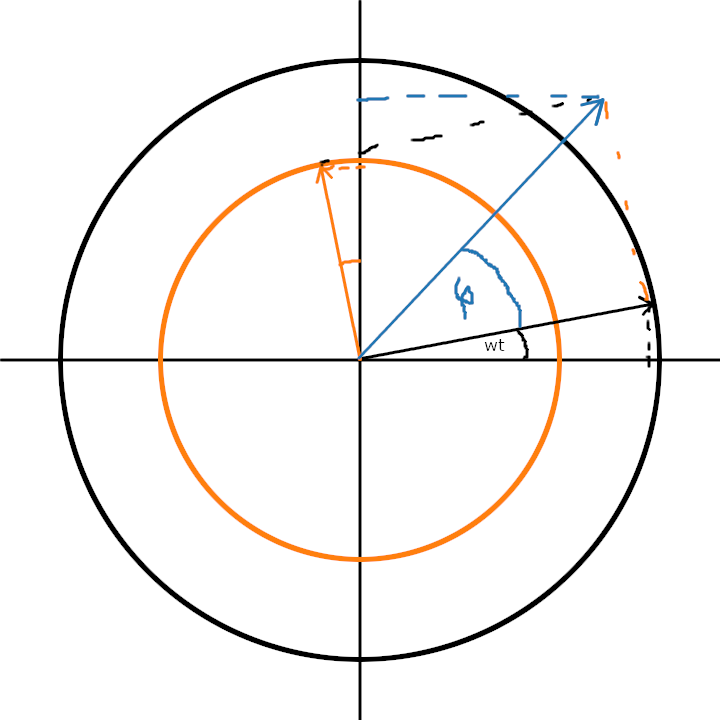
\includegraphics[width=0.4\textwidth]{./bilder/sinus_plus_sinus.png}
	\caption{Veranschaulichung}
	\label{fig:sps}
\end{figure}
\noindent
Jetzt will man ja die Summe beider Sinusfunktionen haben. Das kann man machen, indem man die jeweiligen y-Komponenten der Vektoren zum gegebenen Zeitpunkt addiert. Es werden einfach direkt beide Vektoren addiert und es kommt der blaue Vektor raus, dessen y-Komponente der Summer der Sinusse entspricht. Wenn man das jetzt zu jeder Zeit macht, dreht sich der blaue Vektor mit der selben Frequenz wie die anderen beiden und seine y-Komponente enspricht immer der Summe der Sinusse. \\
\noindent
Der entscheidende Gedanke ist jetzt: Das ist eine eigene Sinusschwingung! Die Amplitude davon ergibt sich über den Pythagoras. Man muss noch beachten, dass der neue Sinus mit einer Phase $\phi$ beginnt zu schwingen und die ergibt sich über $\tan^{-1}(\frac{A}{B})$. Das Ergebnis sieht also so aus:
\begin{align}
\sqrt{A^2 + B^2} \sin \left(\omega t + \tan^{-1}\left( \frac{A}{B} \right) \right) = C \sin(\omega t + \phi)
\end{align}
Wenn die Ausgangssinusse noch Phasen haben, dann ist die Herangehensweise die selbe, es kommen nur noch ein paar Ausdrücke dazu, weil man die eben mit berücksichtigen muss.

\section{Nyquist-Frequenz}
\begin{align}
f_{\text{nyquist}} = \frac{1}{2} \cdot f_s
\end{align}
Sie ist definiert als die halbe Abtastfrequenz (Samplefrequenz). Nach dem dazugehörigen  Abtasttheorem, müssen alle Anteile in einem Signal kleinere Frequenzen haben, als die Nyquist-Frequenz, damit das abgetastete Signal beliebig genau rekonstruiert werden kann. 
\begin{align}
f_{\text{signal}} < f_{\text{nyquist}}
\end{align}
Also muss die Abtastfrequenz größer als doppelt so groß wie die Frequenz das abzurasternden Signals sein.

\section{DFT-Auflösung}
\textit{Dieses Kapitel ist sehr durcheinander}

Die diskrete FT ist erstmal nur eine Abbildung, die eine Liste von komplexen Zahlen in eine andere Liste komplexer Zahlen abbildet unter der Annahme, dass das ``Eingangssignal'' einer Periode eines periodischen Signals entspricht. 
\begin{align}
\label{dft}
G(m) = \sum_{n=0}^{N-1} e^{-2\pi i \frac{kn}{N}} g(n)
\end{align}
Dabei ist $G(m)$ genauso lang wie $g(n)$, nämlich $N$ Einträge. Das ganze findet bisher ohne Rücksicht auf die Auflösung im Messraum statt.
Gleichung \ref{dft} ausgeschrieben ist:
\begin{align}
G(m) = \sum_{n=0}^{N-1} g(n) \left[ \cos \left(2\pi \frac{mn}{N} \right)-i \sin \left( 2\pi \frac{mn}{N}\right) \right]
\end{align}
und man bezeichnet die cosinus und sinus Funktionen in nennt man diskrete Basisfunktionen $C^N_m(n)$ und $S^N_m(n)$. Die inverse DFT sieht ja bis auf das Plus recht ähnlich aus.
Jede der eindimensionalen Basisfunktionen 
\begin{align}
C^N_m(n) &= C^N_n(m) = \cos\left(2\pi \frac{mn}{N} \right) \\
S^N_m(n) &= S^N_n(m) = \sin\left(2\pi \frac{mn}{N} \right) 
\end{align}
Damit sind sie ``periodisch in $N$'': Wenn ich in einer Funktion das Argument durch $N$ teile, dann strecke ich die Fkt um den Faktor $N$. Durch dieses $N$ wird bewirkt, dass eine Periode, welche für $m=1$ genau den Wert 1 hätte, sich nun bis $N$ streckt. Die Frequenz der Funktionen ist also $m/N$ und damit die Kreisfrequenz $\omega_m = 2\pi m /N$. Die Zahl $m$ wird in diesem Beispiel ``Wellenzahl'' genannt.
Wenn jetzt zB $N=8$ und $m=4$, dann benötige ich zur sinnvollen Abrasterung mindestens eine $f_{\text{abtast}} > 2 \frac{m}{M} = 1$Hz.

Da $M$ für $m=1$ die Periode von 1 auf $M$ streckt und $m$ lediglich dafür sorgt, dass in $M$ mehrere Perioden reinpassen, ist $M$ selbst jedoch auch immer noch ein Punkt ab dem sich dann das Signal welches aus den $m$ Perioden besteht wiederholt.

\textit{$M$ ist ja die Anzahl an Samplewerten die ich habe. Wenn ich 1000 Messpunkte habe in meinem Sample, dann ist $M=1000$ und ich weiß zwar nicht nicht genau, woher die Annahme kommt, dass dieses Sample eine Periode eines periodischen Signals darstellt, aber da diese Annahme da ist, ist das so. Das $m$ geht dann seine Werte durch und für jedes $m$ wird $G(m)$ ausgerechnet. Wenn $m=1$, bleibt in den Basisfunktionen nur $2\pi \frac{n}{M}$ stehen, die haben dann die Frequenz $1/M$. Aber bisher wurden noch keine Einheiten betrachtet glaube ich, das heißt ich betrachte auch in welchem Abstand die Werte gesamplet wurden. Sei der Abstand zwischen zwei Samplepunkten $\tau$, dann decken meine $M$ Punkte eine Distanz von $M\tau$ ab (ich dachte erst $(M-1)\tau$, aber die nächste Periode beginnt erst im Abstand $\tau$ vom letzten Samplepunkt).}

\subsection{Welche Frequenz gehört zu welchem $m$?}
\textit{Dieses Kapitel ist sehr durcheinander}
Ich habe genauso viele Werte im Spektrum, wie ich Datenpunkte habe, nämlich $M$ und decke damit eine Zeitspanne von $M\tau$ ab. Für $m=1$ ergibt das für die Basisfkt eine Frequenz von $1/M$. Ist die Frequenz der Basisfunktionen gleichzusetzen mit der Frequenz, zu der die $m$ gehören, also die die \texttt{fftfreq()} liefert? Ich denke nicht, weil die Frequenzen die zu den $m$ gehören über folgendes definiert sind:
\begin{align}
f_m = m \cdot \frac{1}{M\tau}
\end{align}
Die haben also einen Bezug zur Periode des gesamten Samples, welche ja $M\tau$ ist.

Die Frequenzauflösung ist umgekehrt proportional zur Länge des Zeitfensters:
\begin{align}
\Delta f = \frac{1}{M\tau}
\end{align}
und geht damit von $0$ bis $\frac{M-1}{M\tau}$, weil $m$ von $0$ bis $M-1$ geht.

Das Spektrum eines reellwertigen Signals ist symmetrisch um den Ursprung.

\section{DFT in Pyhton}

\subsection{fftfreq}

\section{Zeropadding}
Egal, wie viele zusätzliche Punkte man im Frequenzraum durch hinzufügen von Nullen erhält, erhält man dadurch keinere bessere Frequenzauflösung. Damit meine ich, dass zwei Frequenzen die nahe beieinander liegen erst dann als separater Peaks im Spektrum auftauchen, wenn man mehr Daten der eigentlichen Funktion zum Transformieren nutzt.


Im Bsp mit 1MHz und 1.05MHz: Wenn ich dazu Punkte in einem Sample habe welches 10$\mu s$ abdeckt(also ein $f_s=1e8$Hz) und dazu noch 6000 Samples im selben Abstand per Zeropadding dazufüge, erhöht sich dadurch zwar meine Auflösung im Frequenzraum, jedoch habe ich immer noch nur 1000 Punkte von meiner eigentlichen Funktion und können nur Signale mit Frequenzunterschiede von mehr als 100Khz unterschieden werden (\textit{Das ergibt sich über $\frac{f_s}{N_{\text{fft}}} = \frac{1e8}{1e3} = 1e5 = 100kHz$}). Da die beiden Sinuse sich in ihrer Frequenz jedoch nur um 50kHz unterscheiden, hat man gar nicht die Informationen, um die beiden Peaks getrennt sichtbar zu machen.\\\\
Wenn ich jetzt statt 1000 Datenpunkten 7000 nehme, dann kann ich Frequenzen bis $\frac{1}{1e-8 \cdot 7000} \approx 14285.7$ auflösen. 
\begin{figure}[H]
\centering
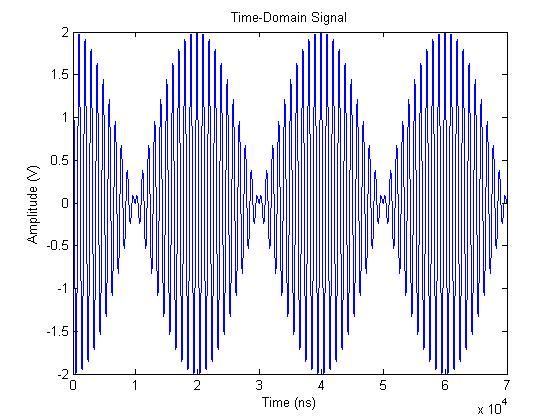
\includegraphics[scale=0.5]{./bilder/td-7000pt-7000fft.jpg}
\caption{Daten}
\label{fig:daten}
\end{figure}
Wenn ich das in dem Beispiel aus Bild \ref{fig:daten} mache, ergibt sich eine DFT mit dem Ausschnitt aus Abb. \ref{fig:dft}.

\begin{figure}[H]
\centering
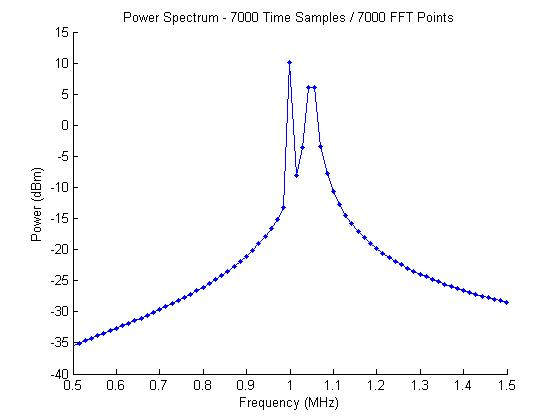
\includegraphics[scale=0.5]{./bilder/fd-7000pt-7000fft.jpg}
\caption{DFT}
\label{fig:dft}
\end{figure}

Man erkennt, dass der Peak bei 1MHz einzeln dargestellt wird, während der bei 1.05MHz auf zwei bins aufgeteilt wird. Das liegt daran, dass wir keinen Punkt bei exakt 1.05 haben. 1Mhz ist ein Vielfaches von 14285.7, da 1Mhz in diesem Bsp auch gerade der Samplingfrequenz entspricht. Das gilt nicht für die 1.05MHz: die nächsten Frequenzen sind 1.043 und 1.057 MHz und daher wird die ``Energie'' gleichermaßen zwischen diesen Bins aufgeteilt. 

Um diesen Problem nun zu lösen, sollten beide Frequenzen bei einzelnen Punkten im Frequenzspektrum liegen. Da wir durch die genügend hohe Samplezahl die Informationen zur Auflösung bereits haben, kann hier nun zeropadding genutzt werden, um die Auflösung zu verfeinern.

\section{Weitere Gedanken}
$\Delta f = \frac{f_s}{N_{\text{fft}}} = \frac{1}{\tau N_{\text{fft}}}$. Das würde bedeuten, dass ich meine Frequenzauflösung dadurch verbessere indem ich meine Samplingfrequenz verringere. Bei gleich bleibender Sampleanzahl würde das bedeuten, dass ich dadurch einen längeren Zeitabschnitt betrachte.

\section{Window functions}
Wenn ich eine Fouriertrafo mache, multipliziere ich durch die Auswahl des Samples meine zu beobachtende Funktion quasi mit einer Rechteckfunktion in dem Bereich des Samples. Diese Windowoperation verändert mein FT-Ergebnis, nämlich in dem Sinne, dass die FT die ich beobachte die Faltung der Frequenzantwort des Windows mit der der eigentlichen Funktion ist. Das Frequenzspektrum einer Rechteckfkt ist ein sinc mit Seitenbändern, welche prominenter sind, wenn das Fenster schmal ist.

\end{document}